\chapter{Flow Control}
During this chapter implementation and evaluation of various control algorithms for flow control purposes will be presented.
\section{Controller Design}
As a first step towards flow control implementation two versions of PI controllers are implemented and compared to each othe ensure stable system behavior. Afterwards, a parallel approach to ILC implementation is used to improve the follow up behavior and reduce control errors.
\subsection{PI Controller}
Measurements similar to static map determination
Different step sizes
\begin{figure}[ht]
  \centering
  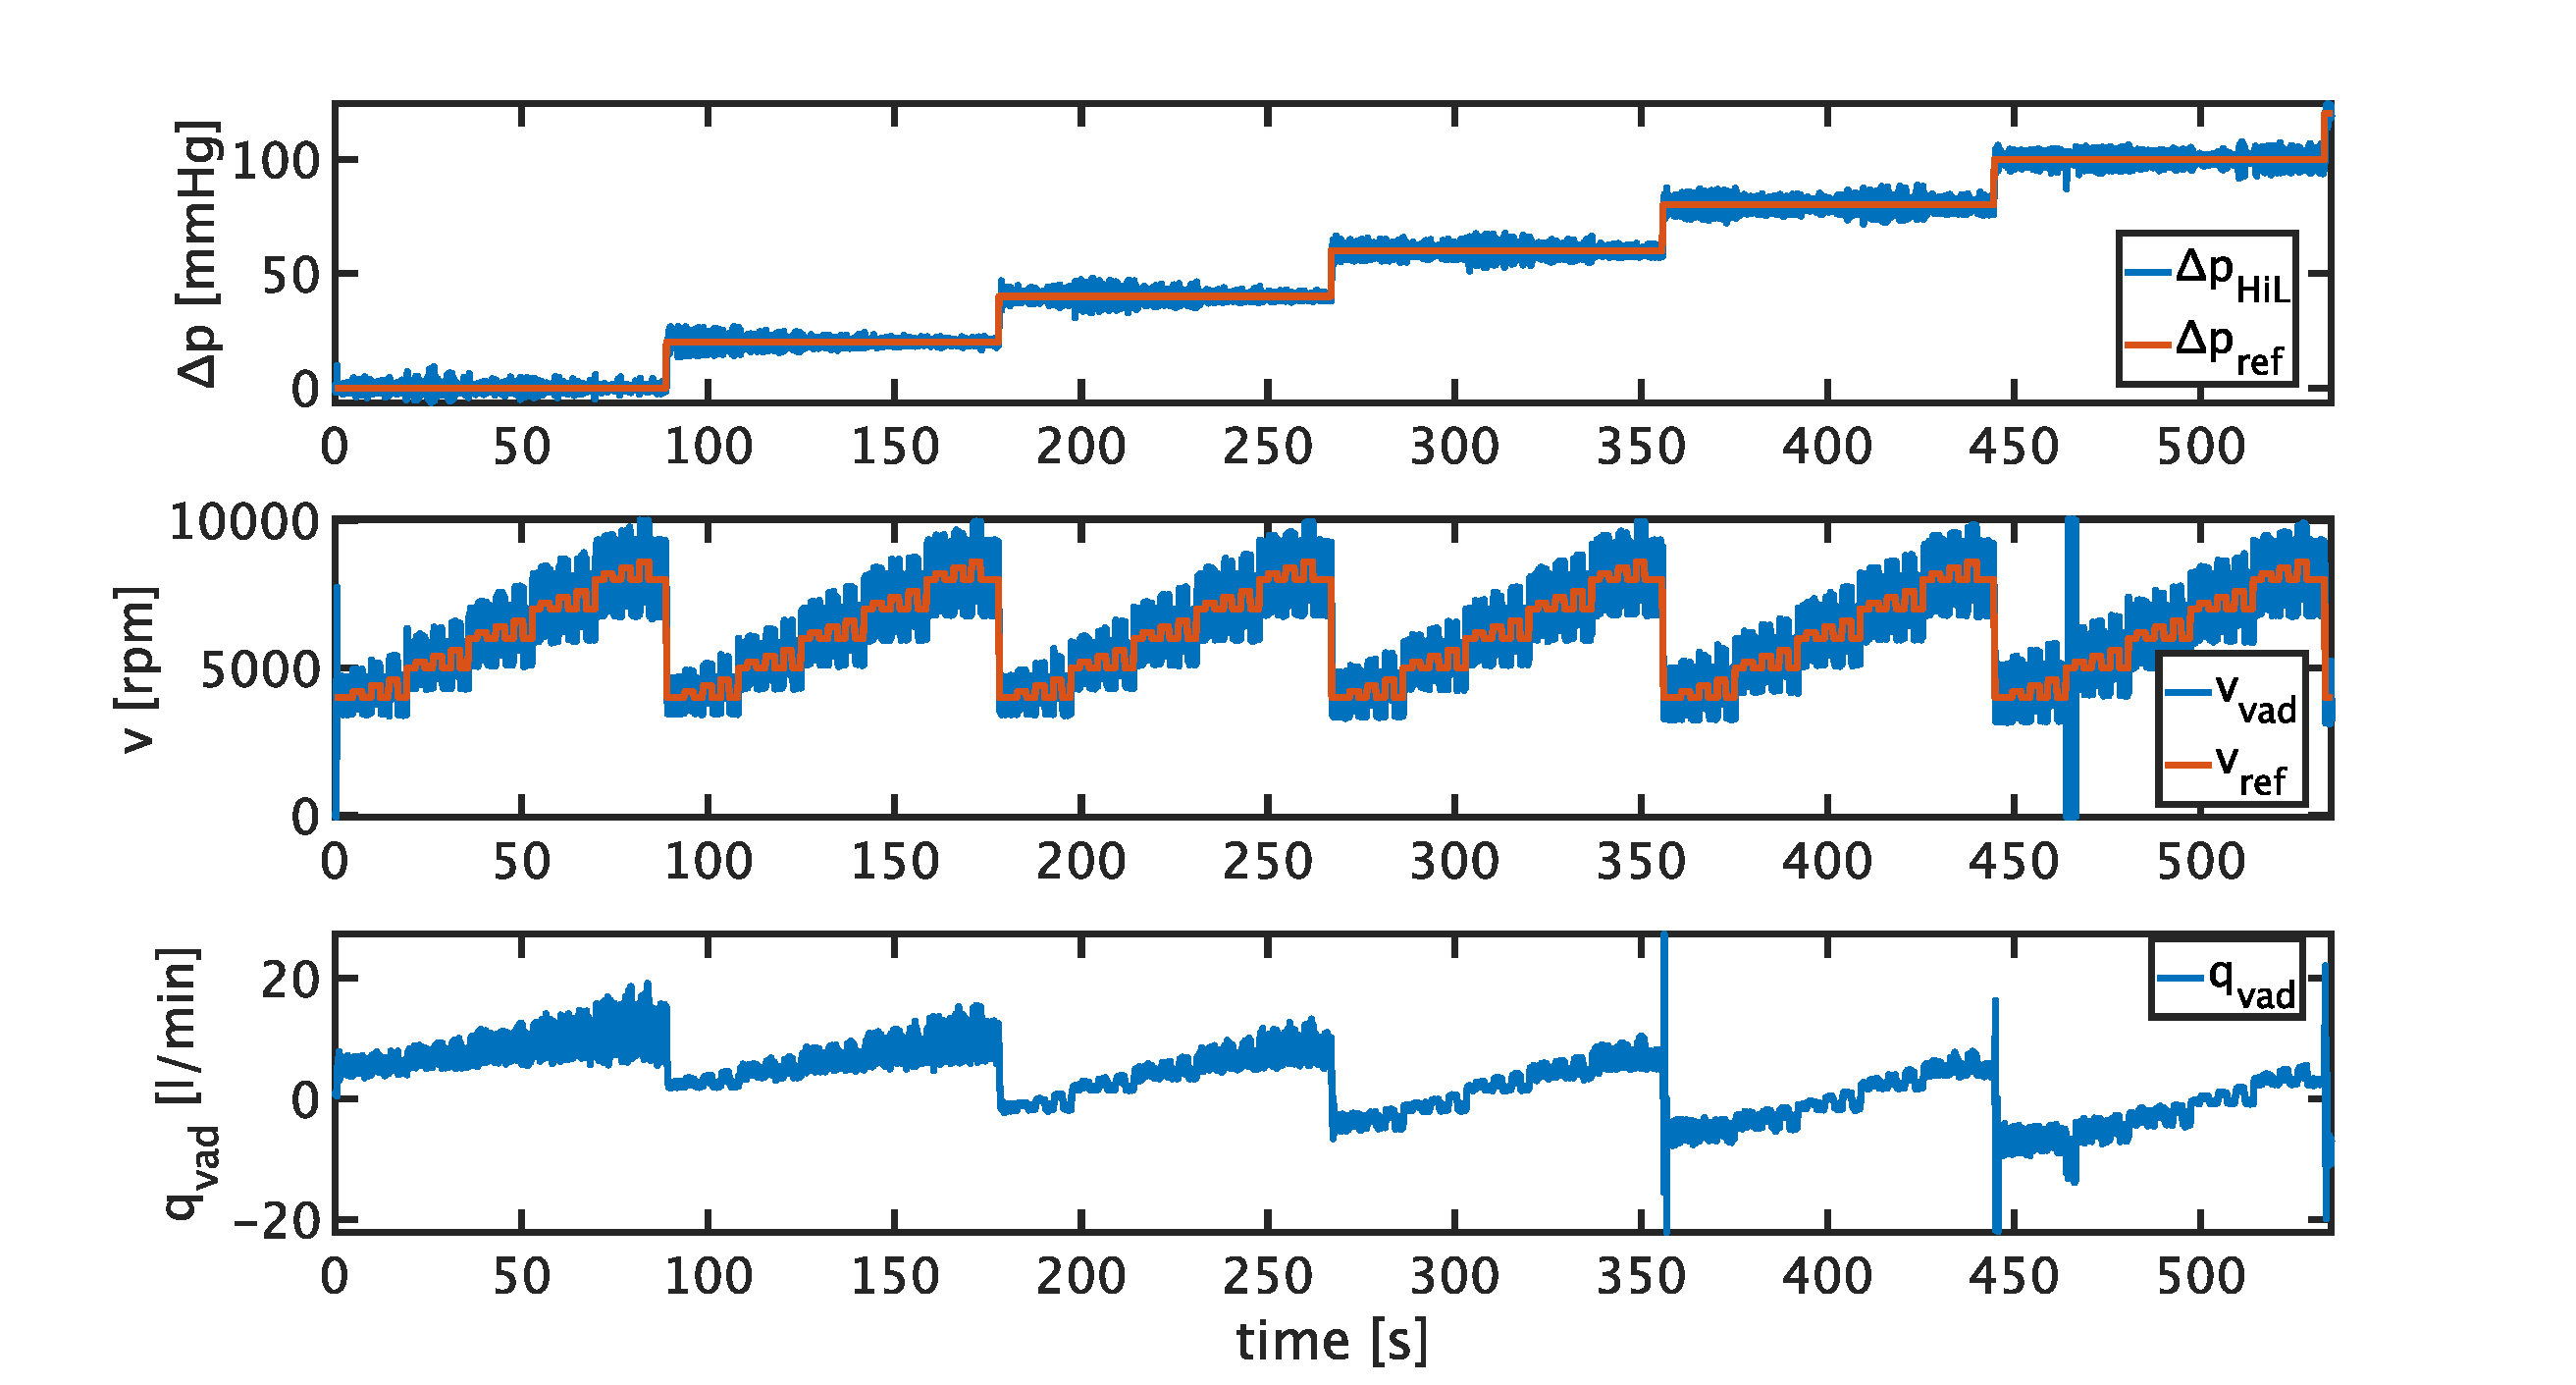
\includegraphics[width=\textwidth]{images/chapt_5/dyn_measure.pdf}
  \caption[Signal curves for determination of PI controller parameters]{Signal curves for determination of PI controller parameters.}
  \label{fig:dyn_meas}
\end{figure}

determination of PI Controller at 40 mmHg


\begin{figure}[ht]
  \centering
  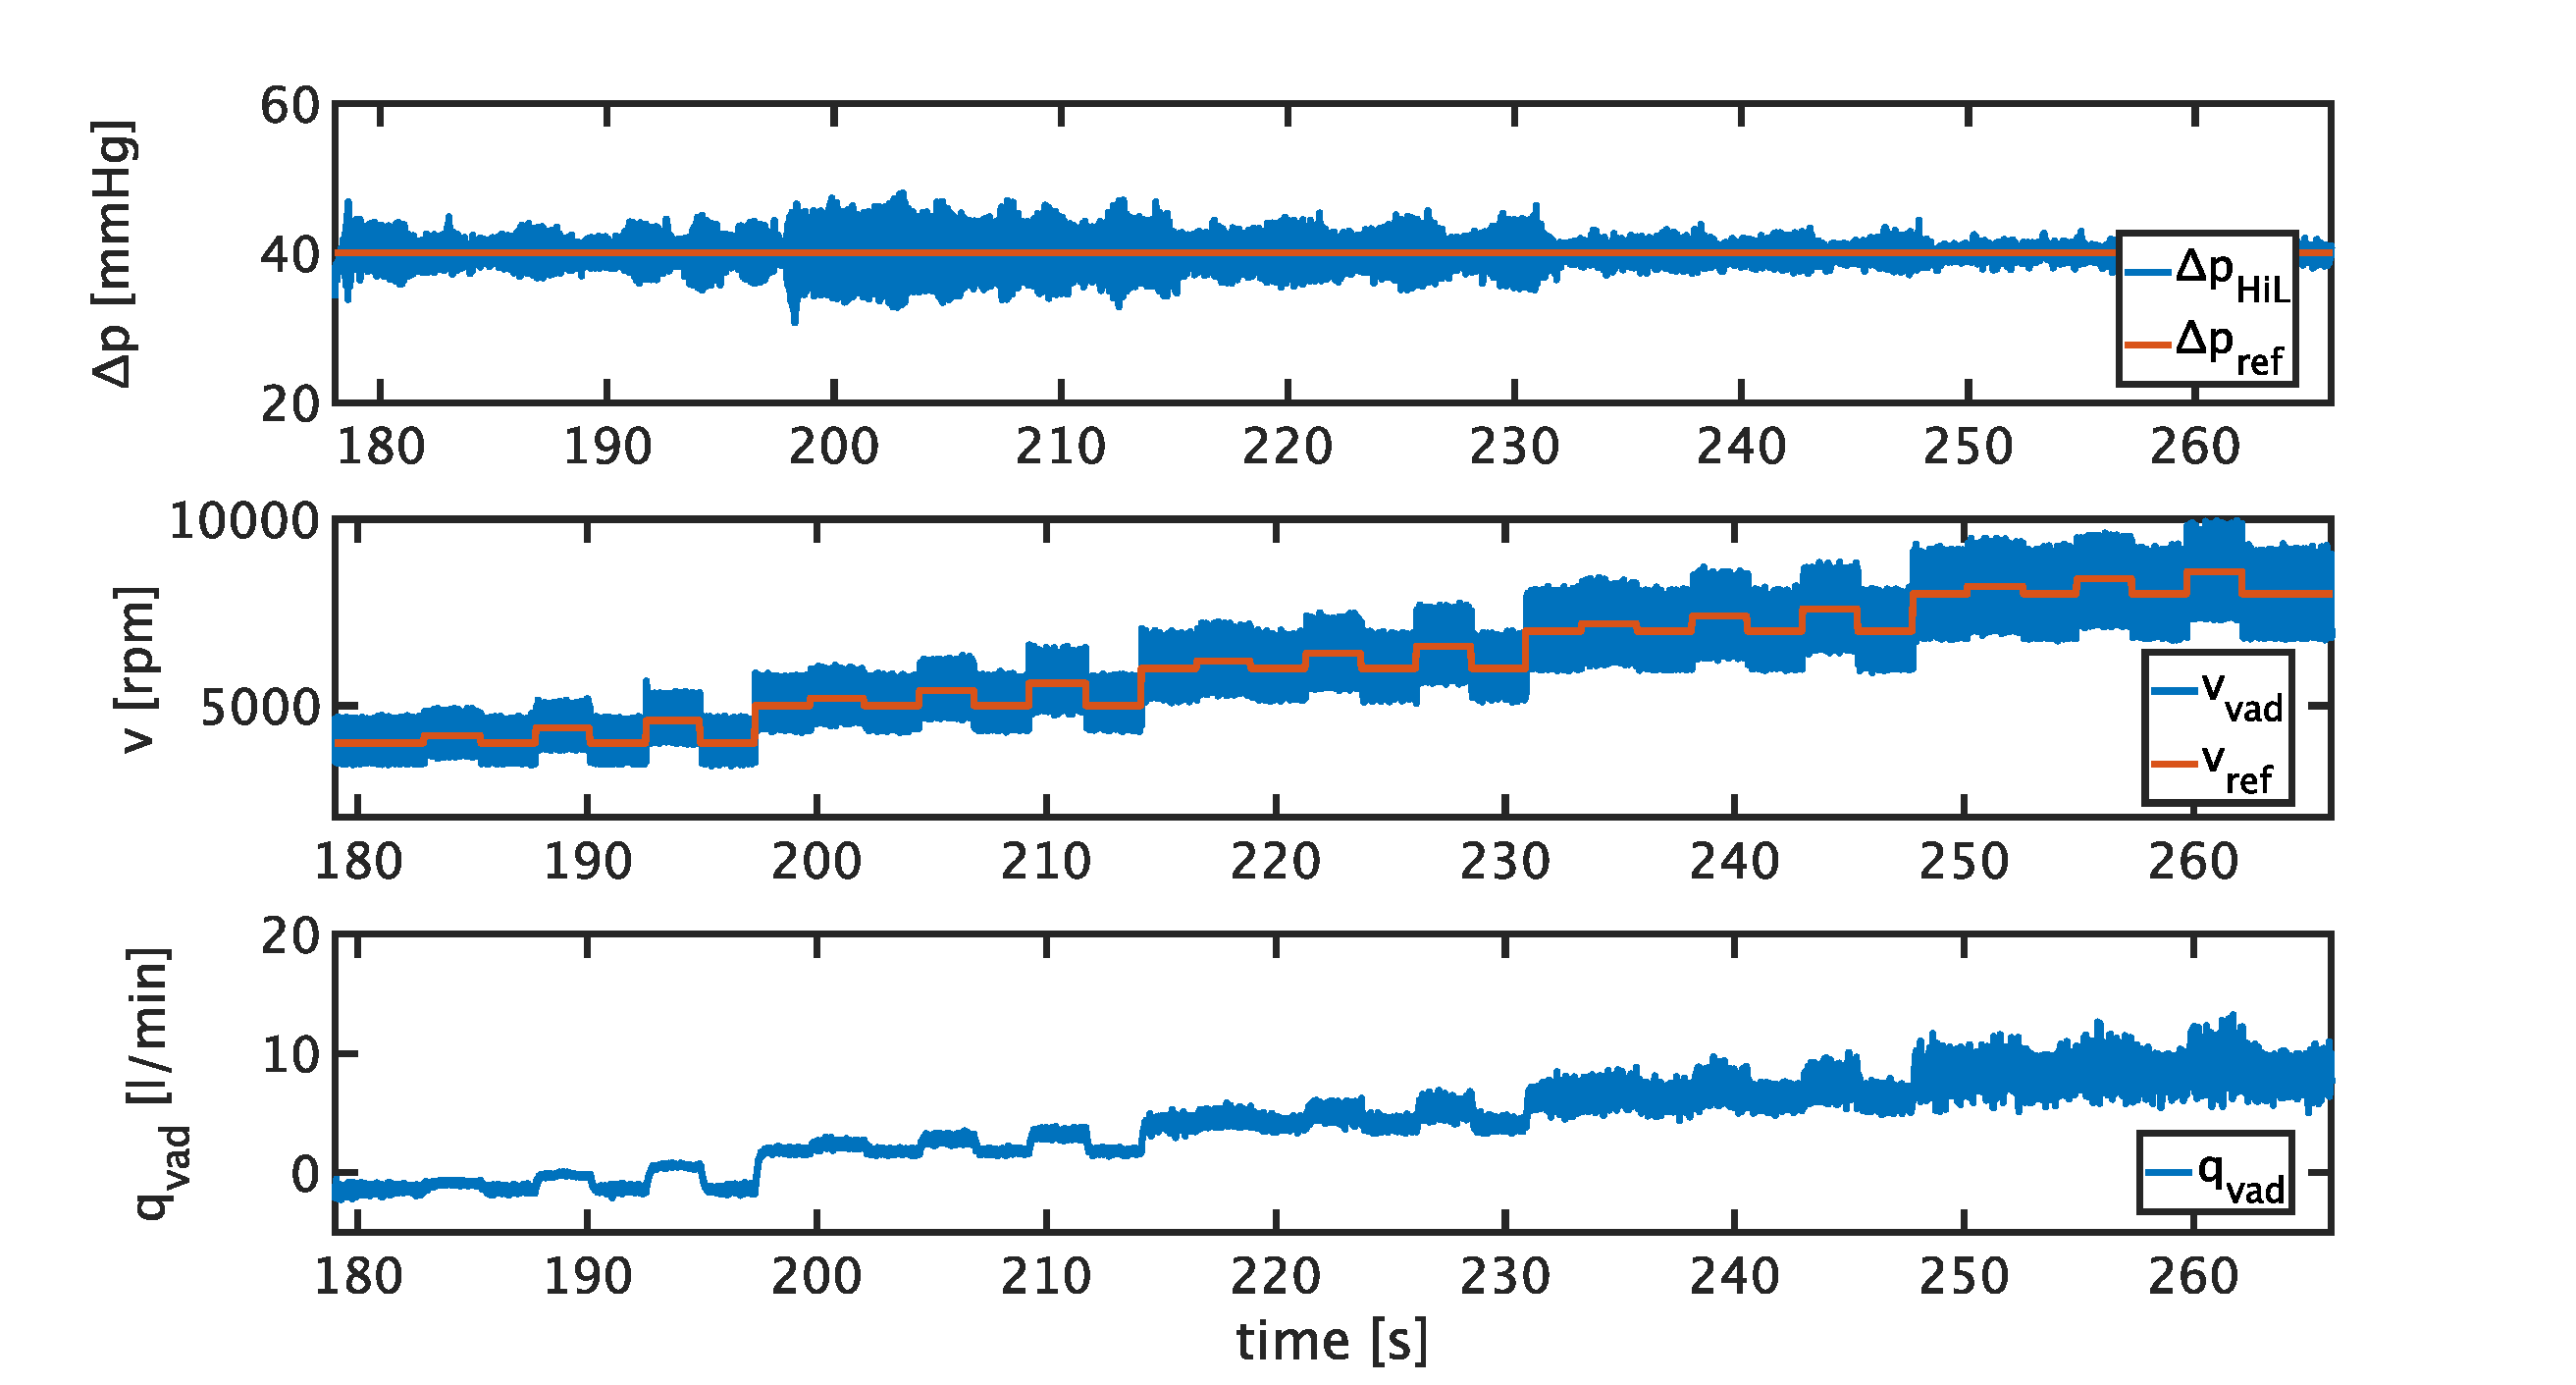
\includegraphics[width=\textwidth]{images/chapt_5/dyn_meas_40.pdf}
  \caption[Signal curves for determination of PI controller parameters at $\Delta{p}=40\,mmHg$]{Signal curves for determination of PI controller parameters at $\Delta{p}=40\,mmHg$.}
  \label{fig:dyn_meas_40}
\end{figure}

for a step from $v_{ref,low}=5000\, rpm$ to $v_{ref,high}=5400\, rpm$.
flow value mit butterworth 8. ordnung fc=5, fs=1000 filtern

\begin{figure}[ht]
  \centering
  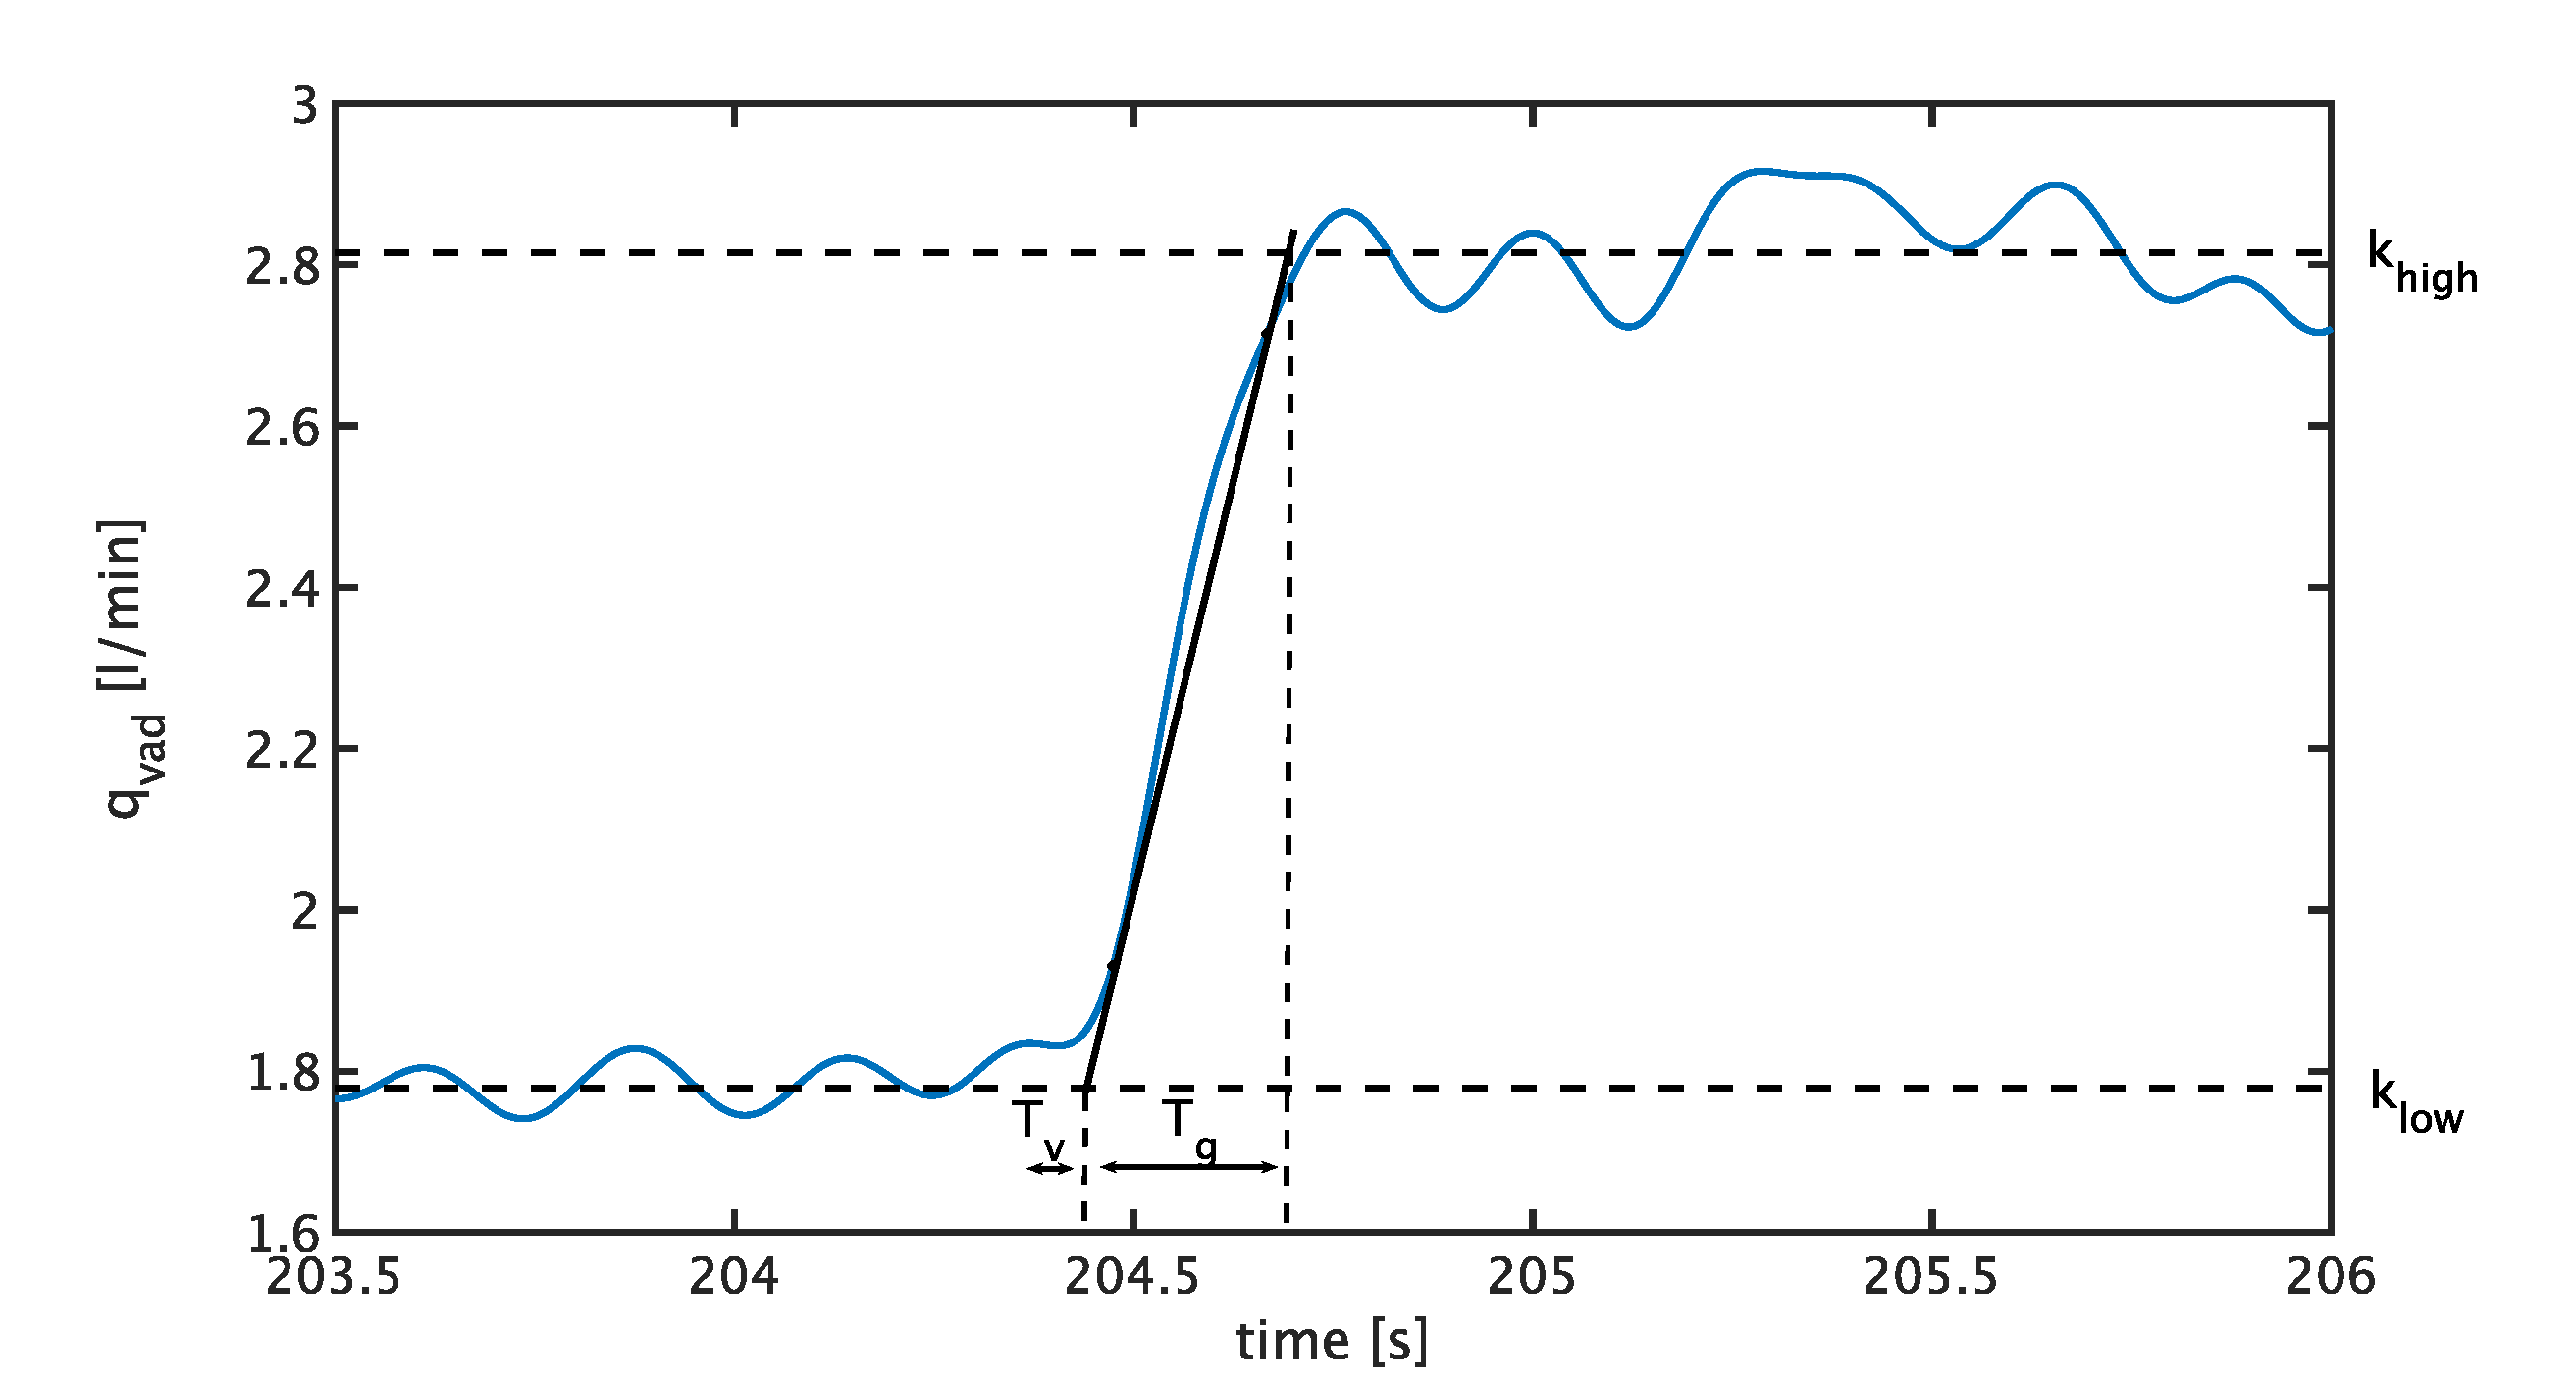
\includegraphics[width=\textwidth]{images/chapt_5/param_calc_PI.pdf}
  \caption[Step response for determination of PI controller tuning parameters]{Step response for a step in rotational speed of $400\,rpm$ for determination of PI controller tuning parameters.}
  \label{fig:param_calc_PI}
\end{figure}

% Dynamische Messung nutzen
% Werte an Sprungstellen
% Nach Wendetangenten verfahren -> GRAFIK
%Berechnung erklären
\subsection{Iterative Learning Control}

\subsection{Iterative Learning Control with varying iteration length}

\section{Evaluation}
\subsection{PI Controller}
gesamt:
rms pi total chr = 0.3705
rms pi total zn = 0.5396
\begin{figure}[ht]
  \centering
  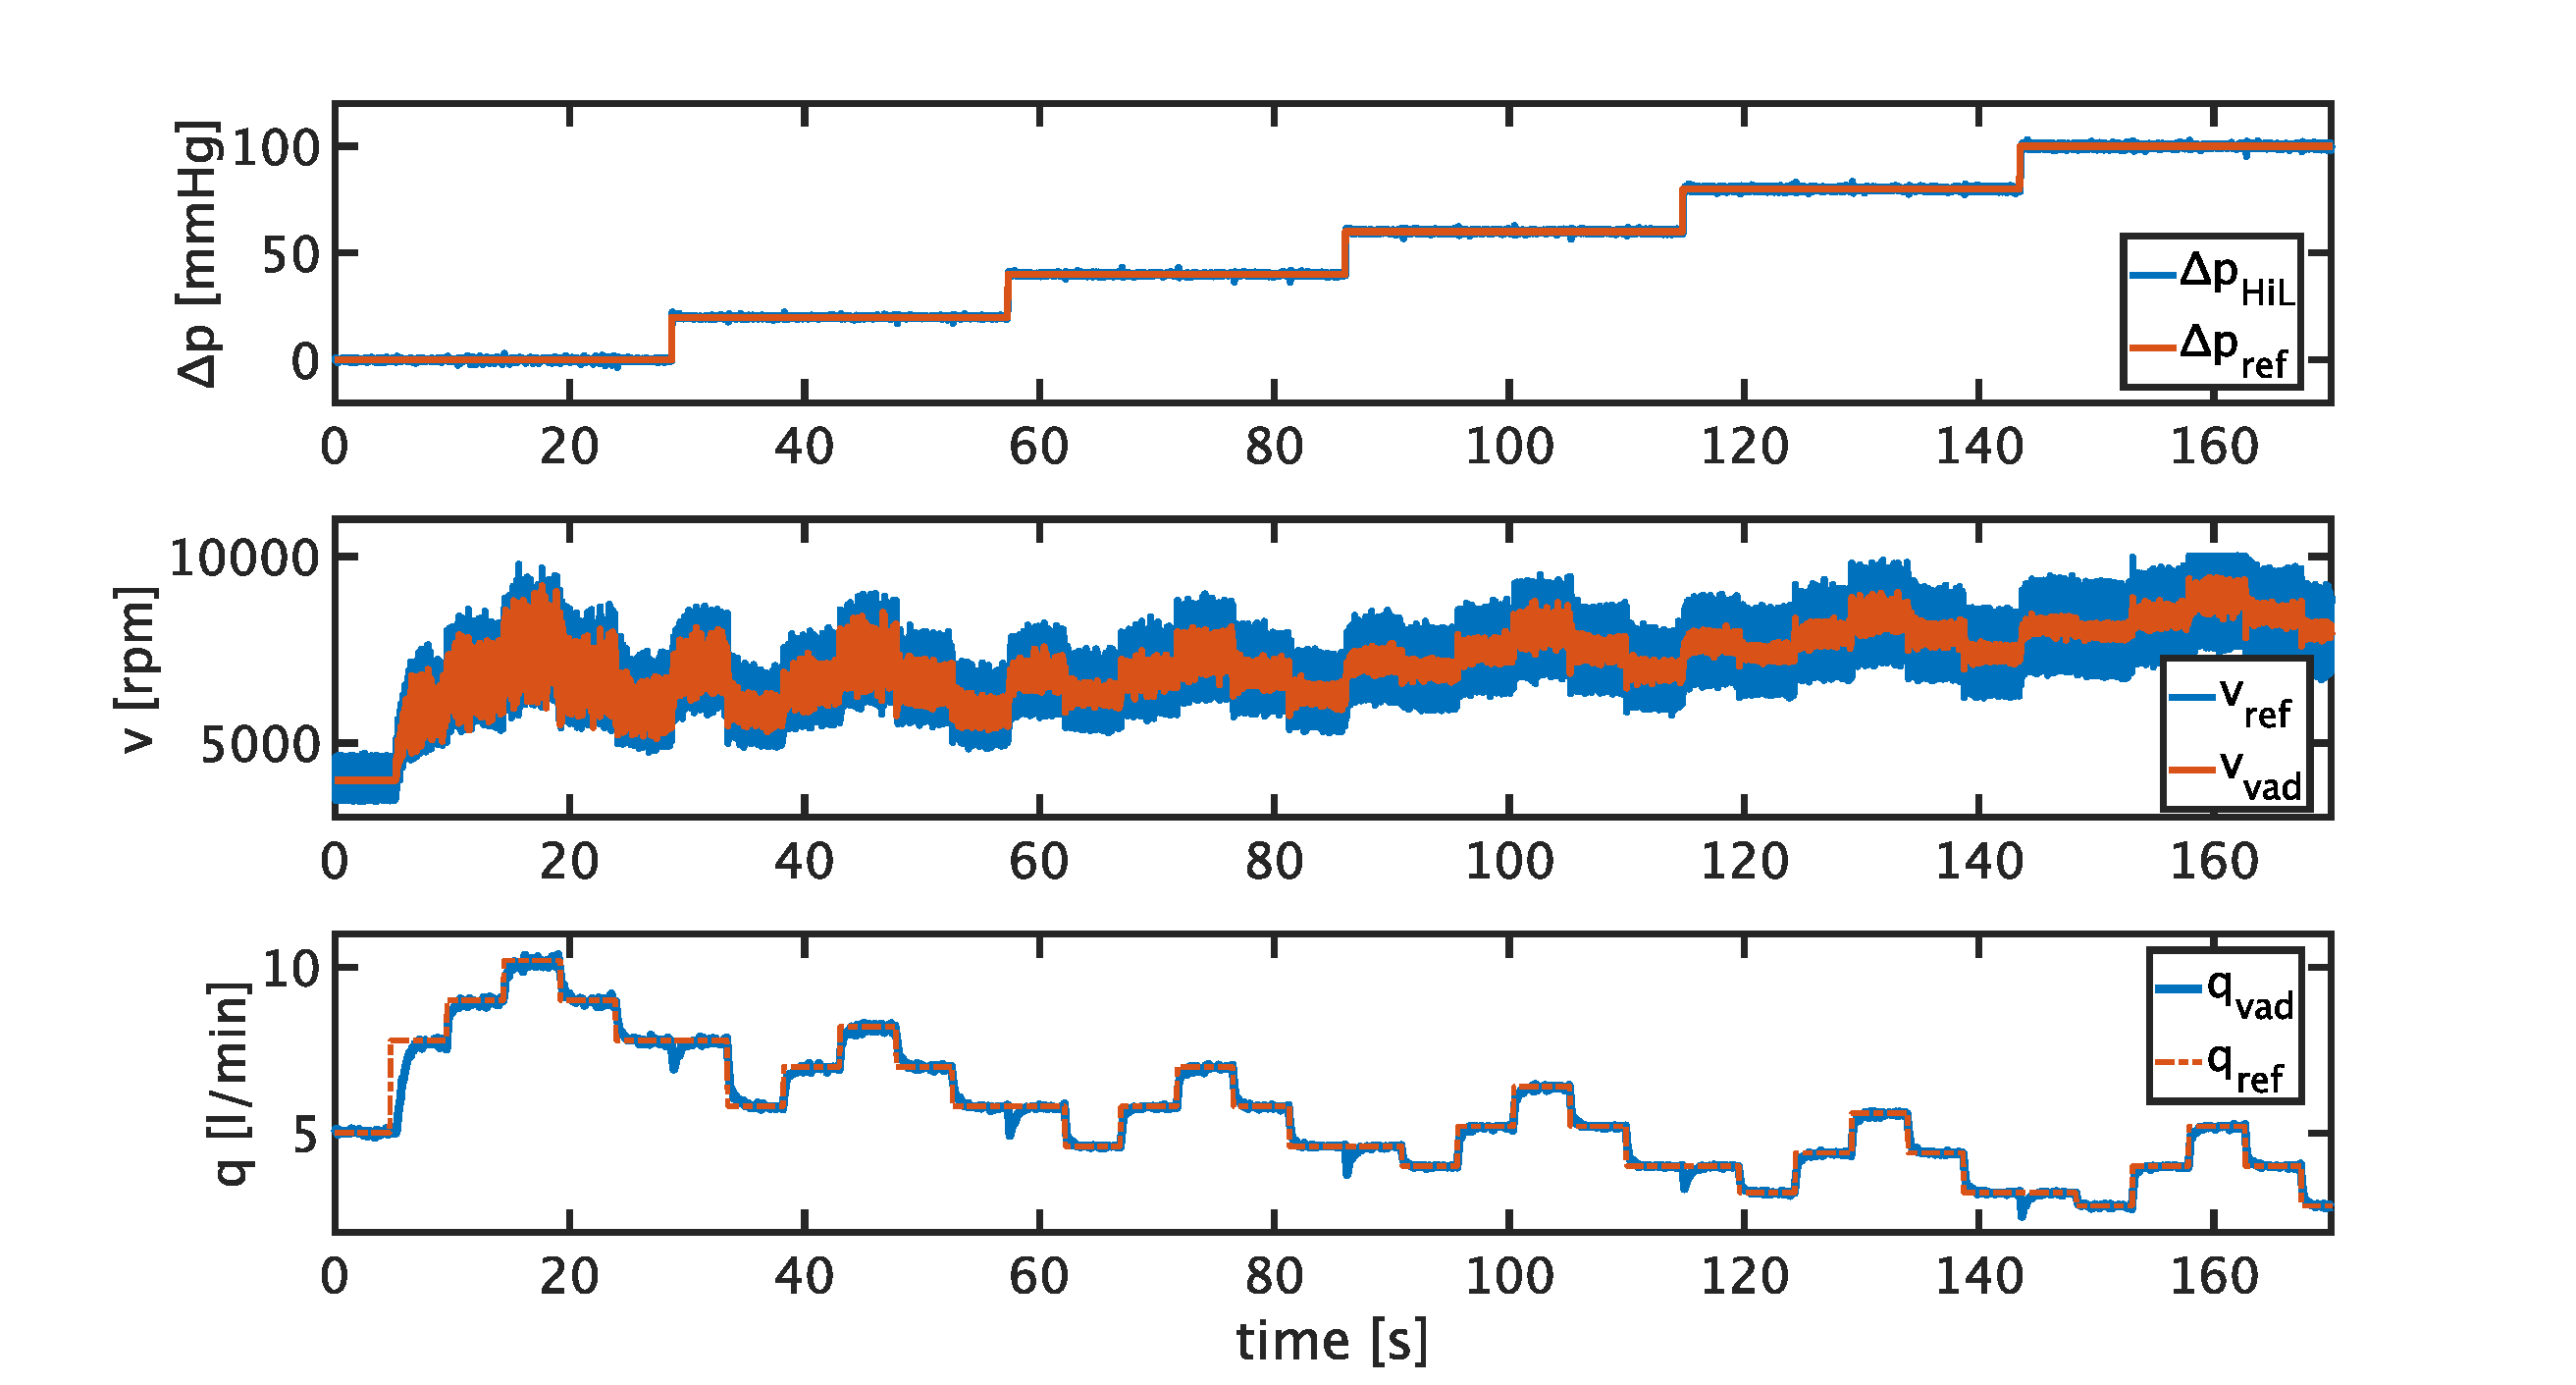
\includegraphics[width=\textwidth]{images/chapt_5/pi_contr_chr.pdf}
  \caption[Step response for determination of PI controller tuning parameters]{Step response for a step in rotational speed of $400\,rpm$ for determination of PI controller tuning parameters.}
  \label{fig:pi_contr_chr}
\end{figure}

% \begin{figure}[ht]
%   \centering
%   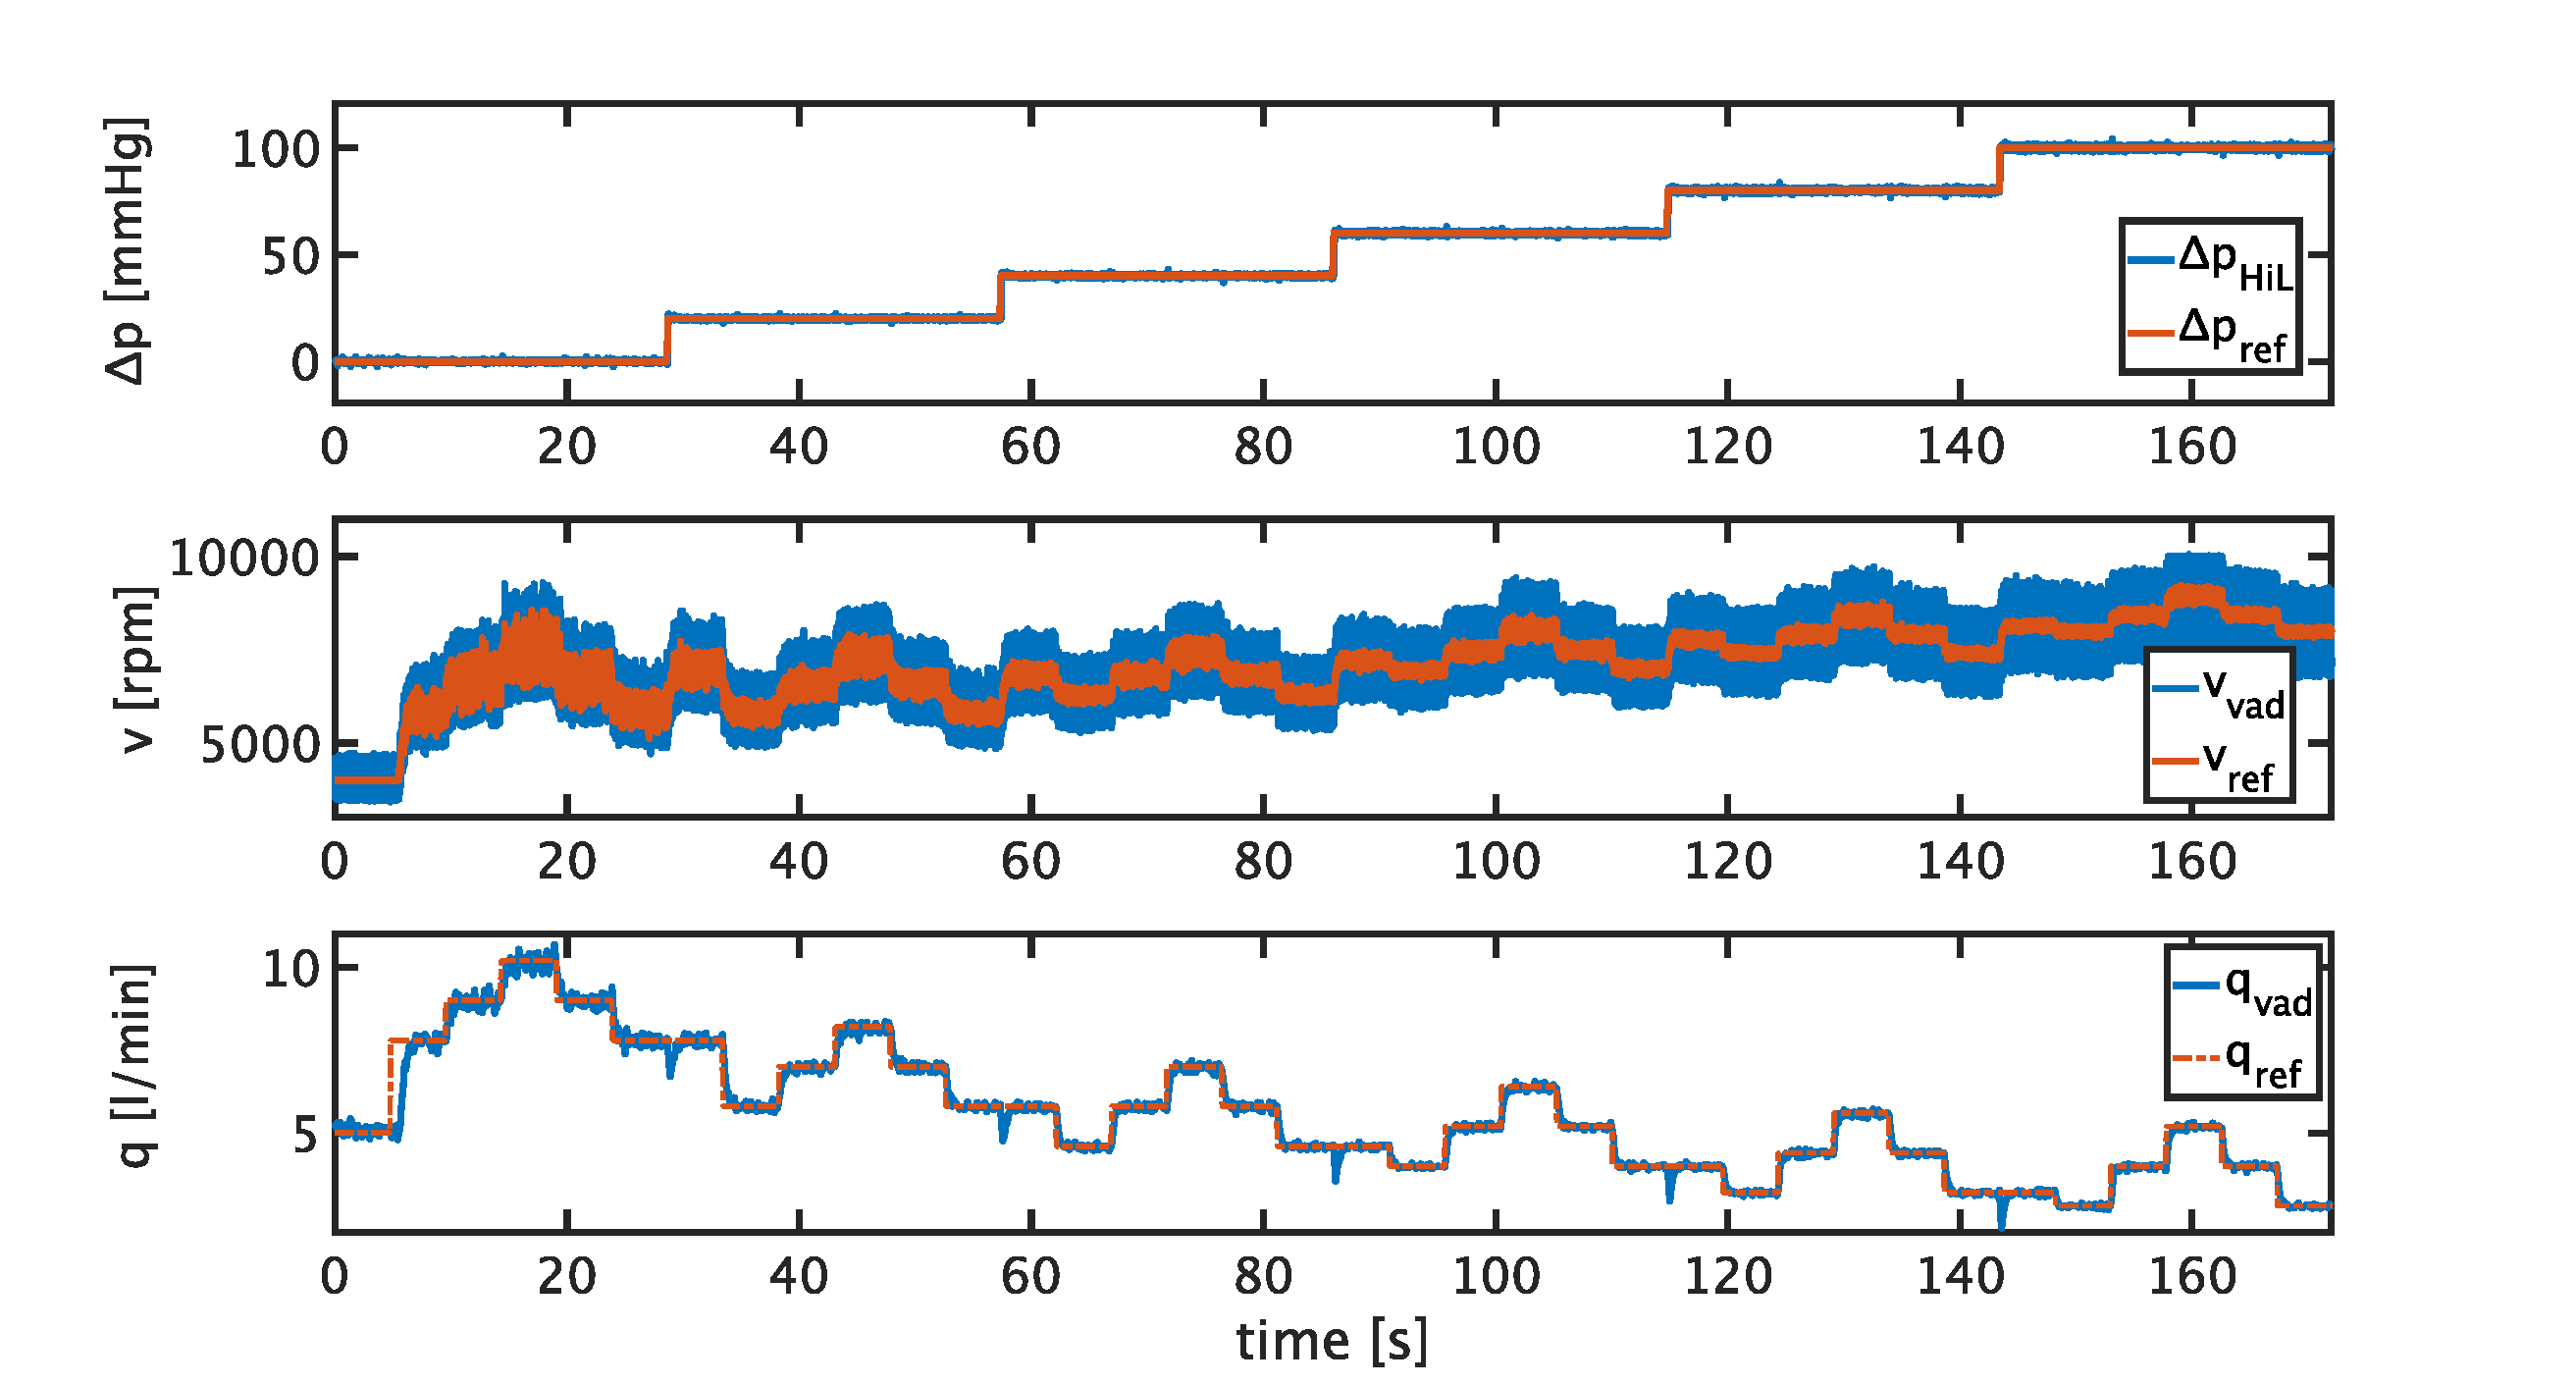
\includegraphics[width=\textwidth]{images/chapt_5/pi_contr_zn.pdf}
%   \caption[Step response for determination of PI controller tuning parameters]{Step response for a step in rotational speed of $400\,rpm$ for determination of PI controller tuning parameters.}
%   \label{fig:pi_contr_zn}
% \end{figure}

Bereich der Auslegung: 40mmHg
RMS PI CHR = 0.2753
RMS PI ZN = 0.4013

% \begin{figure}[ht]
%   \centering
%   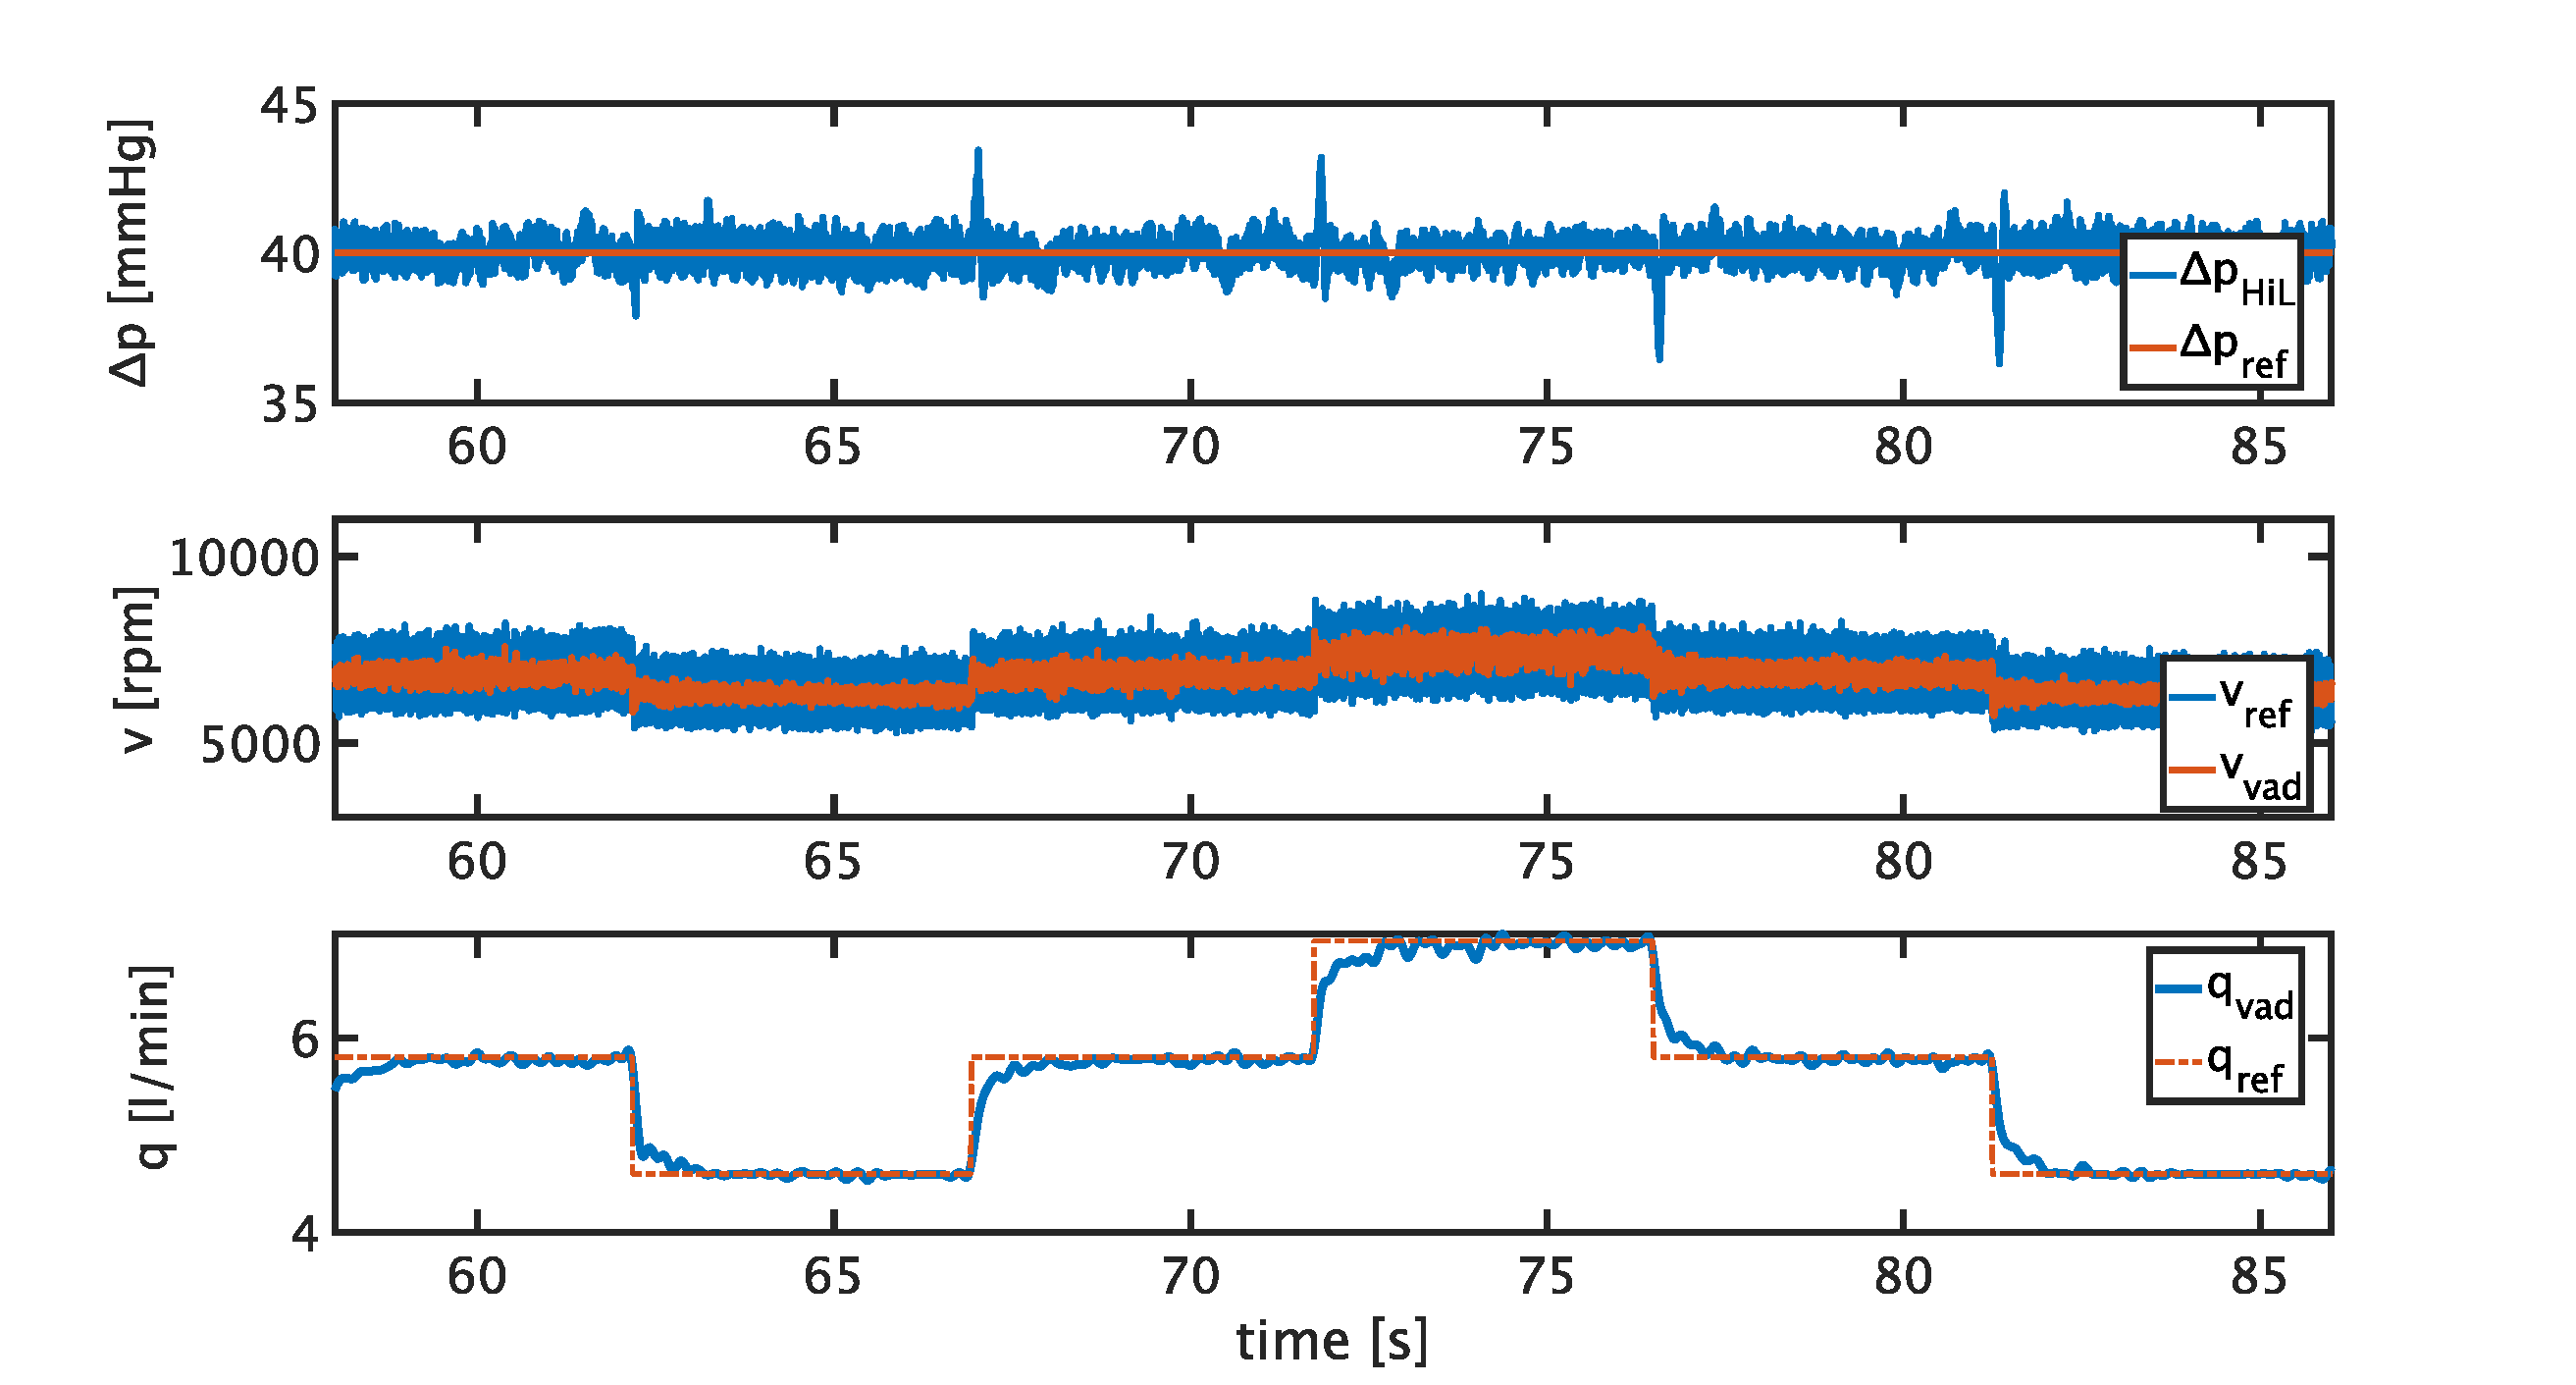
\includegraphics[width=\textwidth]{images/chapt_5/pi_contr_chr_40.pdf}
%   \caption[Step response for determination of PI controller tuning parameters]{Step response for a step in rotational speed of $400\,rpm$ for determination of PI controller tuning parameters.}
%   \label{fig:pi_contr_chr_40}
% \end{figure}

\begin{figure}[ht]
  \centering
  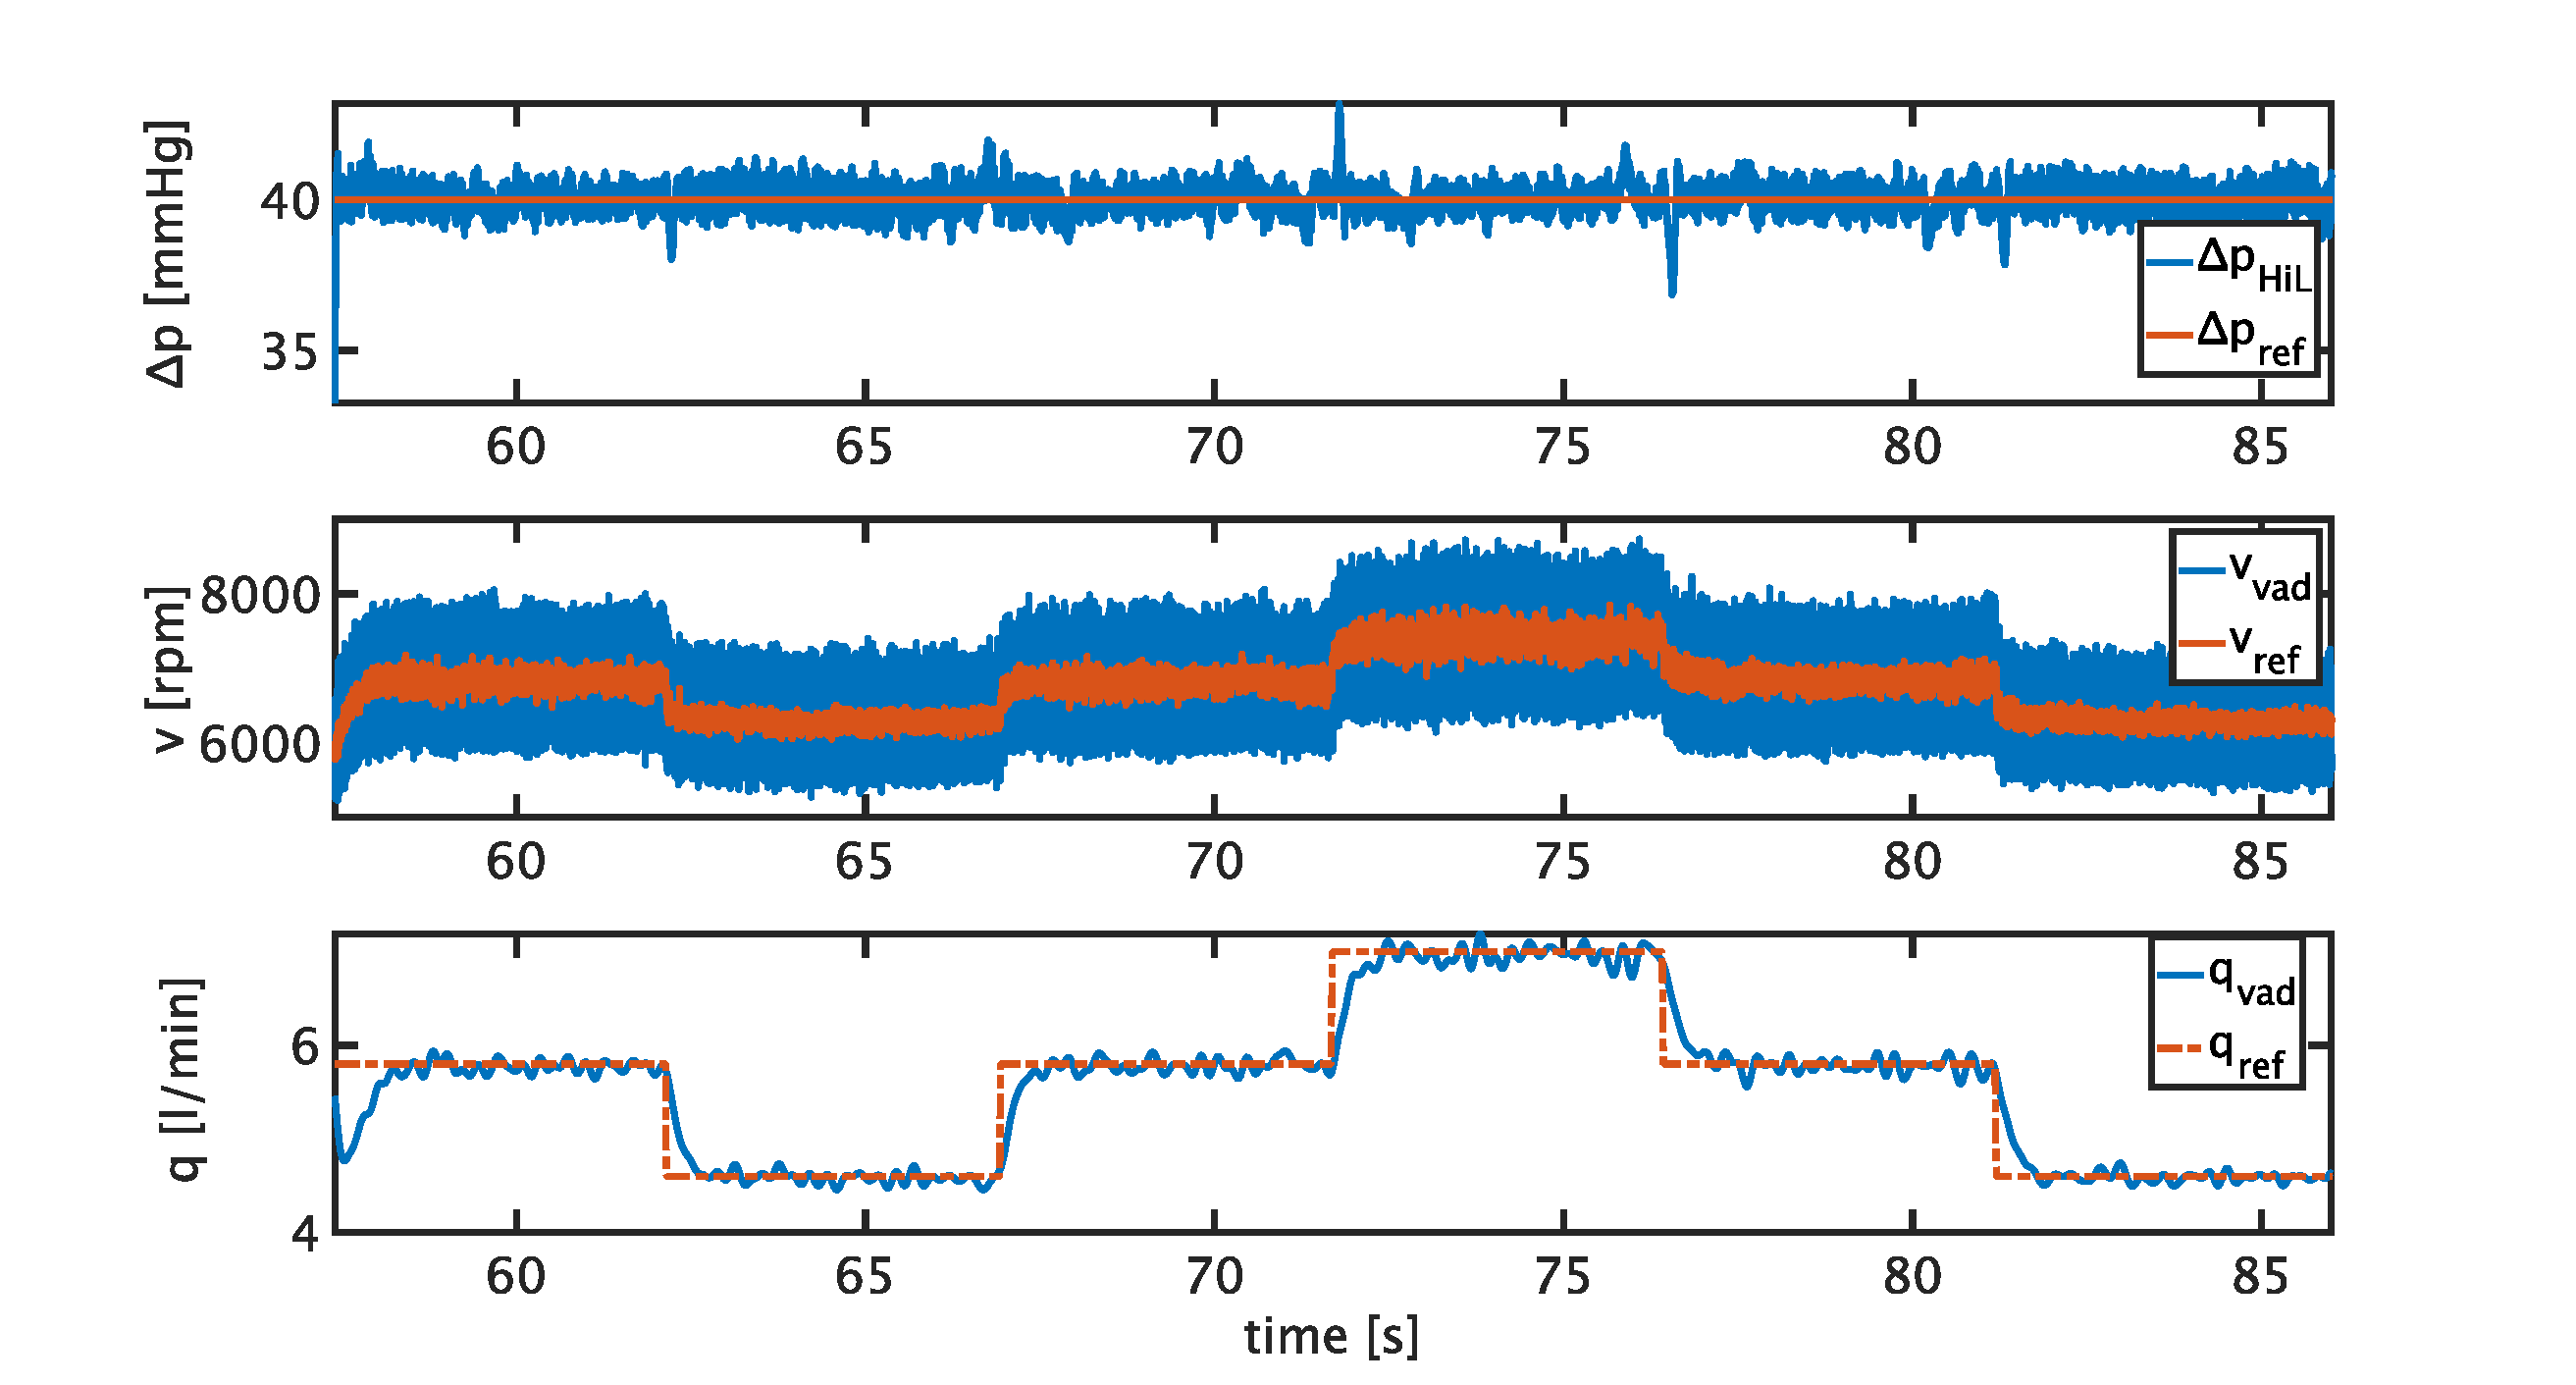
\includegraphics[width=\textwidth]{images/chapt_5/pi_contr_zn_40.pdf}
  \caption[Step response for determination of PI controller tuning parameters]{Step response for a step in rotational speed of $400\,rpm$ for determination of PI controller tuning parameters.}
  \label{fig:pi_contr_zn_40}
\end{figure}
\subsubsection{Chien Hrones Reswick}
% Dynamische Messung nutzen
% Werte an Sprungstellen
% Nach Wendetangenten verfahren -> GRAFIK
%Berechnung erklären
\subsection{Iterative Learning Control}
\subsection{Iterative Learning Control with varying iteration length}
% Kontanten Fluss über verschiedene Druckbereiche?
%
% %Druckverlauf ohne Störung
%
% Herzschlag dazu - Druckverlauf
